%%% app movel - funcionalidade
\begin{frame}{Aplicação Móvel - Funcionalidades}

\vspace*{-3em}

\begin{itemize}
	\item Consultar \textbf{voluntários, organizações, eventos e posts};
	\item permitir o registo e autenticação de voluntários através da aplicação;
	\item possibilitar aos utilizadores autenticados interagir com a plataforma (realização de \textit{posts}, seguimentos de outros utilizadores, etc.).
\end{itemize}

\end{frame}

%%% app movel - arquitetura
\begin{frame}{Aplicação Móvel - Arquitetura}
	
\vspace*{-4em}
	
\begin{itemize}
	\item \textbf{UI}: define interfaces de utilizador e trata operações de \textit{input};
	\item \textbf{Model}: define DTO's (\textit{Data Transfer Objects}) e implementação de Cache;
	\item \textbf{API}: funciona como \textit{proxy} da \textit{web} API.
\end{itemize}	

\centering
\scalebox{0.40}{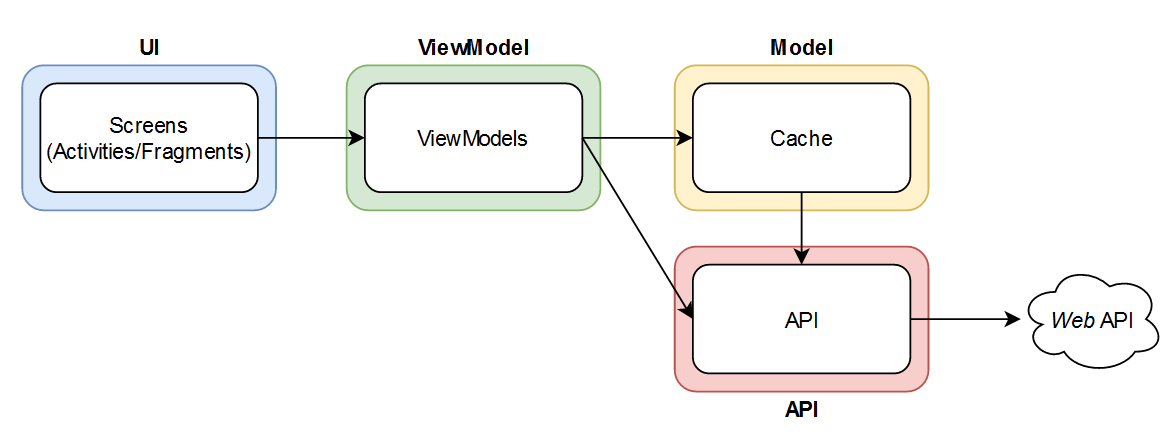
\includegraphics{Figures/mobile_app_architecture}}\\

{\small Arquitetura da aplicação móvel.}

\end{frame}